\documentclass[12pt,a4paper,onecolumn]{article}
\usepackage[utf8]{inputenc}
\usepackage{amsmath}
\usepackage{amsfonts}
\usepackage{amssymb}
\usepackage{graphicx}
\usepackage[margin=1in]{geometry}
\usepackage{mathpazo}
\usepackage{float}

\usepackage{color}
\usepackage{hyperref}
\hypersetup{
    colorlinks=true,
    linkcolor=black,
    urlcolor=red,
    linktoc=all
}
\usepackage[toc,page]{appendix}

\addtocontents{toc}{\protect\hypertarget{toc}{}}
\usepackage{algorithmic}
\usepackage{newunicodechar}
\newunicodechar{fi}{fi}
\newunicodechar{fl}{fl}

\author{Anya Chaturvedi \\ Sagar Sahni \and K. R. Prajwal \\ Ketaki Vaidya  }
\title{%
  The Capacitated K-Centre Problem\\
  \large Summer Internship Report 
  }
 \date{}
\begin{document}
\begin{titlepage}

\newcommand{\HRule}{\rule{\linewidth}{0.5mm}} 

\center 

%\textsc{\LARGE Capacitated K-Centre Problem}\\[1.5cm] % Name of your university/college
% Minor heading such as course title



\HRule \\[0.4cm]
{ \huge \bfseries Capacitated K-Centre Problem}\\[0.4cm] % Title of your document
\HRule \\[1cm]
 \textsc{\Large Summer Internship Report}\\[1cm] % Major heading such as course name
{\large May $9^{th}$ - July $11^{th}$, 2016}\\[0.5cm]
%----------------------------------------------------------------------------------------
%   AUTHOR SECTION
%----------------------------------------------------------------------------------------

\includegraphics[scale=0.06]{iitd_logo.png}\\[0.5cm] % Include a department/university logo - this will require the graphicx package
\textsc{\large Indian Institute of Technology, Delhi}\\[9cm] 


 % Date, change the \today to a set date if you want to be precise

%----------------------------------------------------------------------------------------
%   LOGO SECTION
%----------------------------------------------------------------------------------------


 \begin{minipage}{0.4\textwidth}
\begin{flushleft} \large
\emph{\\Authors:}\\
Anya Chaturvedi\\
K.R. Prajwal\\
Sagar Sahni\\
Ketaki Vaidya
 % Your name
\end{flushleft}
\end{minipage}
~
\begin{minipage}{0.4\textwidth}
\begin{flushright} \large
\emph{Supervisor:} \\
Dr. Naveen Garg \\
Professor\\
Dept. of CSE\\
IIT Delhi % Supervisor's Name
\end{flushright}
\end{minipage}\\[2cm]
%----------------------------------------------------------------------------------------

\vfill % Fill the rest of the page with whitespace



%\section[Abstract]{Abstract \begin{flushright}\hyperlink{toc}{TOC}\end{flushright}}
\newpage
\thispagestyle{empty}

\begin{center}

\large{Department of Computer Science and Engineering}\\[0.5cm]
\normalsize
\textsc{Indian Institute of Technology Delhi}\\[2.0cm]

\LARGE Certificate\\[1 cm]

\end{center}
\normalsize \begin{flushleft}
This is to certify that the students whose names are given below have done their summer internship on \textbf{The Capacitated K-Centre Problem} under my guidance \\for a duration of two months  in Summer - 2016  and have submitted this report.
\end{flushleft}
\vspace{0.5cm}
\begin{table}[h]
\centering
\begin{tabular}{lr}
 Name & Institute \\
\\
Anya Chaturvedi & Motilal Nehru National Institute of Technology, Allahabad \\ 
K.R. Prajwal &  National Institute of Technology, Tiruchirappalli \\
Sagar Sahni & SRM University, Kattankulathur \\
Ketaki Vaidya & National Institute of Technology, Silchar
\end{tabular}
\end{table}

\vspace{4cm}



 \begin{minipage}{0.4\textwidth}
\begin{flushleft} \large
\emph{\\Date:}\\

\end{flushleft}
\end{minipage}
~
\begin{minipage}{0.4\textwidth}
\begin{flushright} 

\large Dr. Naveen Garg \\
(Supervisor)% Supervisor's Name
\end{flushright}
\end{minipage}\\[2cm]



\newpage
\thispagestyle{empty}

\begin{center}


\LARGE ACKNOWLEDGEMENTS\\[2 cm]

\end{center}
\large \begin{flushleft}
We wish to express our sincere gratitude to Professor Naveen Garg for letting us be a part of his research group for the summer.\end{flushleft}
\begin{flushleft}We also wish to thank the research scholars, Jatin, Aounon and Nikhil for their continuous  help and guidance in carrying out our implementations and giving us topics to brainstorm upon.\end{flushleft} \begin{flushleft}Thank you to all the above mentioned for taking out time for us and providing us with an enriching and memorable experience.\end{flushleft} \begin{flushleft}

 - Anya, Prajwal, Sagar \& Ketaki.
\end{flushleft}

\end{titlepage}

\tableofcontents


\section{Abstract}
The capacitated $K$-centre problem is basically a facility location problem, where one is asked to assign $K$ points to $K$ facilities in a given distance metric. In doing this we minimise
the maximum distance from a vertex to the facility to which it is assigned while keeping in mind that each facility may be assigned at most $L$ vertices including itself. This problem is known to be NP-hard.

We show our attempts at solving this problem, counterexamples that we studied and a few basic implementations of the same. Starting with a more formal description of our problem, we describe the flow method which helps us verify a solution to the problem. Next, we show how we implemented the integer program and a partially correct local search algorithm. In implementing the above programs we have used three ways for making the input graphs. One is a random graph, second a more clustered form i.e. a star graph, and the last one is generated by taking points in a unit square. Other than this we have included a few observations which may not be very conclusive but are our attempts to solve the problem over the summer.
\section{A Look at the Problem}
The problem studied by us is actually a generalization of the $K$-centre problem which we explain here. 
\subsection{The $K$-Centre Problem}
Given $n$ vertices with specified distances, one wants to build $K$ facilities at different vertices such that each vertex has access to a facility and minimise the maximum distance between each vertex and the corresponding facility. This problem is NP-hard. An approximation algorithm with a factor of $\eta$, for a minimization problem, is a polynomial time algorithm that guarantees a solution with cost at most $\eta$ times the cost of an optimal solution. For the basic $K$-centre, methods have been presented for obtaining an approximation factor of 2. Given a complete undirected graph $G$ = $(V, E)$ with distances $d(v_i, v_j) \in \mathbb{N}$ satisfying the triangle inequality, we have to find a subset $S \subseteq V$ such that $|S| = k$ and such that it covers all $V$.\\\\
 \textbf{Input:}\\1. A metric space, or, in other words, a complete graph that satisfies the triangle inequality.\\2. An upper bound on the number of centres, $K$.\\\\
\textbf{Output:}\\
$$\min_{S \subseteq V}\max_{v \in V}\min_{s \in S}d(v,s)$$
where $d$ is the distance function.

This is quite similar to the problem of placing $K$ disks such that all points are covered in the set $V$ and the maximum radius required to do so is minimised.

\subsection{The Capacitated K-Centre}
The capacitated $K$-centre problem is nothing but a generalization of the $K$-centre problem. We have to
output a set of at most $K$ centres, as well as an assignment of vertices to centres. No more than $L$ vertices may be assigned to a single centre. Under these constraints, we
wish to minimise the maximum distance between a vertex $u$ and its assigned centre
$\varphi (u)$. \\\\
\textbf{Input:}\\1. A metric space, or, in other words, a complete graph that satisfies the triangle inequality.\\2. An
upper bound on the number of centres, $K$.\\3. A maximum capacity for each centre, $L$.\\\\
\textbf{Output:}\\
$$ \min_{S \subseteq V}\max_{u \in V}d(u,\varphi(u)) $$such that,   $$|\{u|\varphi(u) = v\}|\leq L \forall v \in S,$$\\where,   $$\varphi : V \rightarrow S.$$\\
The first constant factor polynomial time approximation
algorithm for this problem was with an approximation factor of 10. Later, a 6-approximation was found which is the best up till date while a 5-approximation works when we can assign multiple centres at any single vertex without counting the center itself while calculating the capacity used.

Initially we went through the sections 2.6 and 9.3 of Williamson \& Shmoys which solve the problem of finding the minimum degree spanning tree problem which is also NP-hard. Here we learnt of methods like local search used to create approximation algorithms. Next we read a few papers related to our problem and gathered what is presented in the upcoming sections.
\section{Checking the Feasibility of the Input Graph}
We say that if we solve the capacitated $K$-centre problem then it will be equivalent to getting the minimum value of $W$ for which $G(W$) has a capacitated dominating set of size $K$, where $G(W)$ refers to the graph having all edges with edge weight less than or equal to $W$.

We can easily set up such an equivalence if we slightly modify our problem. Given a graph $G = (V,E)$ and a capacity function $c : V \rightarrow N$ we say that $S \subseteq V$ is a capacitated dominating set if there exists a mapping $f : V \rightarrow S$ (domination mapping) such that:\begin{enumerate}

\item $\forall v \in V ,\:\forall s \in S,\:f(v) = s \Longrightarrow (v,s) \in E$\\ \item $\forall s \in S,\:| \{ v \in V| f(v) = s \} | \leq c(s)$
\end{enumerate}In the new version of the $K$-centre problem, the goal is to get a set $S$ of $K$ vertices and an assignment $h : V \rightarrow S$ of every vertex (in $V$) to an open centre such that the greatest distance between a vertex and the centre it is assigned to is minimised and no facility is assigned more vertices than its capacity. Note that the assignment is not for all vertices in $V$. We make the assumption that every centre serves itself and the capacity $(L(v))$ of a vertex $v \in V$ is the maximum number of clients it can serve (excluding itself). 

Now we can say that solving the capacitated $K$-centre problem is equivalent to getting the minimum value of $W$ for which $G(W)$ has a capacitated dominating set of size $K$. 
$S \subseteq V$ is an optimal solution to the capacitated $K$-centre problem if and only if $w(S)$ is the minimum value of $W$ for which the graph $G(W)$ has a capacitated dominating set of size $K$.
It is also easy to verify that a capacitated dominating set of size $K$ in $G(w(S))^i$, for some $i$ and some optimal solution $S$, forms an $i$-approximation for the $K$-centre problem.

However, note that the capacitated dominating set problem is an NP-complete problem. Therefore, we cannot get a capacitated dominating set of size $K$ in polynomial time, unless $P = NP$. Similar to the uncapacitated version, the capacitated version too is hard to approximate within a factor of 2.
\subsection{Verification using a Network Flow }
Given a graph $G = (V,E)$ and a capacity function $c : V \rightarrow N$, checking whether $S \in V$ is a capacitated dominating set can be viewed as a network problem. We construct a directed graph $G_S = (V_S,E_S)$ as follows:\begin{enumerate} 
\item $V_S = V \cup \{s,t\}$
\item $E_S = \{(s,v_i) | v_i \in V \} \cup \{(s_i,t) | s_i \in S \}\cup \{(v_i,s_i) | v_i \in V \wedge s_i \in S \wedge (v_i,s_i) \in E \}$\end{enumerate} Let $c_S : E_S \rightarrow N\mathbb{N}$ be the capacity function such that, $$c_S(e_{uv}) =\left\{ \begin{array}{cc}c(u),  &  v = t \\\\ 1, & otherwise \end{array}\right.$$
As defined above, in the final graph $G_S$ we add two more vertices s (source) and t (sink) to the vertex set of G. We add directed edges from s to all vertices in $V$, from each vertex in $V$ to its neighbours in $S$ and each vertex in $S$ to $t$. We take the capacity function to be equal to the capacity of the source vertex for edges incident on $t$ and to be equal to 1 for every other edge in $E_S$. \\
The flow network as described has been shown in Figure 1.
\begin{flushleft}
 \begin{figure}[H]
 \begin{center}
 \includegraphics[scale=0.5]{diag2.jpg}
 \end{center}
  \caption{The flow network}
  \label{Figure 1}
\end{figure}
\end{flushleft}
  Now it is easy to verify that, S is a capacitated dominating set in G if and only if $G_S$ has a maximum coverage of $|V|$ from $s$ to $t$ equal to the total vertices in the graph. 

\section{The Integer Program}
Linear programming is a mathematical technique for maximising or minimising a linear function of several variables such as output or cost. The decision variables with respect to which the optimum is obtained can come out to be fractional or integral. An integer programming problem is a mathematical optimization or feasibility program in which
some or all of the variables are restricted to be integers which makes it a subset of linear programming. Ours is a problem where we
wish to minimise the maximum distance between a vertex u and its assigned centre thus our integer program is framed as:
\\




\textbf{Objective Function:}\\
\hspace{15mm} $$z=\sum_{i=1}^{N}cen[i]$$
\\
\textbf{Variables:}\begin{enumerate}
\item \textit{\textbf{cen}} - an integer dictionary which specifies the centres among the vertices
where if $cen[i]=1$ then the $i^{th}$ index vertex is taken to be a centre otherwise not.\item \textit{\textbf{assignments}} - a dictionary, $assignments[i][j]=1$ will represent that the $j^th$ index vertex is assigned to the centre created at the $i^th$ index vertex, we initialise it with the adjacency matrix
\item \textit{\textbf{$N$}} - the total number of vertices
\item \textit{\textbf{$adj$}} - a dictionary which stores the adjacency matrix of the graph 
\end{enumerate}
\textbf{Constraints:}
\begin{enumerate}
\item $\forall i \sum_{j=1}^{N}assignments[i][j]\leq L*cen[i]$\\\hspace{1cm}\ldots makes sure no more than $L$ vertices are assigned to a centre
\item $\forall j \sum_{i=1}^{N}assignments[i][j] = 1$\\\hspace{1cm}\ldots a vertex can be assigned only to a single centre
\item $\forall i \, \forall j \, assignments[i][j] \leq cen[i]$\\\hspace{1cm}\ldots a vertex can only be assigned to a vertex if the later is a centre
\item $\forall i , \forall j \, assignments[i][j] \leq adj[i][j]$\\\hspace{1cm}\ldots 
assignment of vertices can only be done if the edge between a vertex and its corresponding centre is present in the original graph

\end{enumerate}

You can refer to the code in Appendix A.

\section{Local Search Algorithm}
Local search can be used on problems that can be formulated as finding a solution by maximising a criterion among a number of candidate solutions.
A local search algorithm starts from a candidate solution and then iteratively moves to a neighbour solution. We move from solution to solution in the space of candidate solutions (the search space) by applying local changes, until a solution optimal is found.
We have used a local search algorithm which was formed by Aounon which is actually a randomised algorithm. It does not work on a set of graphs but by increasing the number of iterations on the same graph it gradually gives the solution for most as the probability involved increases.

Here, we start with a set $S$ of random $K$ vertices in graph $G$ . Let $S$ be the set of all $K$ vertex sets which are formed by replacing one vertex in $S$ by a vertex in $V$ (one-swap vertex sets). We look for the set in $S$ which maximises the number of dominated vertices. If one of the set dominates more vertices than current $S$ then we set $S$ to that set and continue the process till we have reached a local optima. We do the assignments through a network flow graph.\\\\\\
\textbf{Algorithm:}
\begin{algorithmic}[1]
\STATE $S \leftarrow {v1, v2,…., vk}$
\STATE $S' \leftarrow {one-swap\: vertex\: sets\: of\: S}$
\WHILE {$MaxFlow(G_{V_{max}}, c_{V_{max}}) > MaxFlow(G_S,c_S)$}
\STATE $S \leftarrow V_{max}$
\STATE $S' \leftarrow {one-swap\: vertex\: sets \: of\: S}$
\STATE $V_{max} \leftarrow argmax _{V \in S} MaxFlow(G_V , c_V )$
\ENDWHILE 
\IF{$MaxFlow(G_S , c_S) = n - k$}
\FORALL {$v \in V$}
\IF{$f_{max}(v,s)=1$}
\STATE $h(v) = s$
\ENDIF
\ENDFOR
\RETURN $S, h$
\ENDIF
\end{algorithmic}


You can refer to the code in Appendix B.






\section{Graph Generation}
\subsection{Random Graph}
For testing the implemented algorithms on random graphs, SNAP, a Python based system developed by Stanford University was used. It takes the number of nodes and edges as input and gives a random sub graph of a data set which we convert represents to an adjacency matrix, ready to be fed into the Integer Program and local search algorithm.

You can refer to the code in Appendix C.

\subsection{Star Graph}
In an attempt to try our programs on a more clustered data set, this program was implemented to create sparsely-connected star graphs, with edges chosen to be added with a probability p.

We were able to get 100\% accuracy and this was the strongest dataset we tested upon.

You can refer to the code in Appendix D.

\subsection{Unit Square}
On discussing our above mentioned methods with Sir he suggested another way for making the input graphs which he felt might give us better  results for further analysis. 
The method proceeds by taking $N$ random points in a unit square.
The edge weight between all possible pairs of these $N$ points are calculated by using different $L^p$ norms, for $p \geq 1$.
$W$ is chosen which denotes the maximum edge weight allowed in a particular thus reducing the number of edges in the otherwise obtained complete graph. 
The graph is built with the $N$ random points as nodes and edges $(a,b)$ if distance between $(a,b)$ is $\leq W$, for all $a,b$ $\in$ $N$. 
This graph is used to obtain the optimal $K$ using a capacity, which we have taken as $L = N/10$.

We have used the same graph to check if the randomised local search algorithm yields the optimal solution with the above obtained $K$ and $L$.


Even though this did not strike at first on why this will be in any manner be different than using random graphs, still we decided to proceed with the implementation. During our visualization of the graphs created, we saw that this method gave us a very large variety of graphs, in the sense that the graphs had local clusters, articulation points, isolated vertices, cliques and a wide variation in the degrees of the nodes.

We checked it on the integer program, local search and randomised local search programs. Mostly it worked but took a long time as we have iterate the local search for 5-10 iterations to increase the chance of it being successful. If somehow the complexity can be reduced we can see how well it works for larger graphs. The complexity as of now is the order of O($n^7$). At present it is working very well for below 40 nodes giving almost a 100\% accuracy but after we clocked it up to 80 nodes(we could not increase more) we found that the accuracy drops sharply to 98-99\%  i.e. one or two failures for every 110 nodes. Though it gives failure few times it is difficult to analyse due to the large number of vertices in the failed examples. 

 Further, we came up with minor hacks and tweaks to get the best of randomization and non-randomization in our algorithm by including them in a single run and could get all correct on several test sets of 110 unit square graphs each. However, this still exists as a minor tweak, and we are not able to analyse pictorially for larger graphs such as 80 nodes as we did for $\leq 40$ nodes. We hence, tried a different approach of representing it as a bipartite graph, but that was not possible through the networkx library which we have used. We hence would need a better method to analyse large graphs of 80 nodes or more.

You can refer to the code in Appendix E.
\section{Observations made}
This section is a collection of all our trials and errors during our exploration of this topic along with few of the concepts learnt which provide the base for these trials.
\subsection{Lower Bound on K}
Let us say we make disjoint set of partitions of our input graph nodes such that each partition has two types of vertices, inner and boundary. The inner vertices are the ones which have no edges with vertices outside their partition, while the boundary vertices are the ones which do have edges to other partitions. Let the $i^{th}$ partition be represented by its inner vertices $C_i$ and its boundary vertices as $B(C_i)$.

Since we know K vertices can cover up to L vertices so the maximum vertices that can be covered is $V = K*L$. Hence the minimum $K$ required to cover $V$ vertices is $\lceil V/L\rceil$. This is a naive lower bound on $K$. But using this concept, we may get a better lower bound. 

Here, in the partitioning as described above, for the vertices other than the boundary vertices we can say that they can only be covered by vertices of their own partition thus we need to open centres in the partition itself for such vertices. If we say there are $p$ partitions then $\sum_{i=1}^{p}\lceil (C_i-B(C_i))/L\rceil$ vertices are required at least to cover the graph and hence this comes to be a lower bound. \\The above bound has been presented in a research paper already. We observed that, the above mentioned paper is not involving the boundary vertices in formulating a lower bound. So, we toyed for some time with ideas on involving the boundary vertices. We thought using the residual capacity, i.e. $\lceil (C_i-B(C_i))/L\rceil*L-(C_i-B(C_i))$ we may be able to cover some or even all of the boundary vertices. Through this we can decide opening more centres or shifting the centres so as to cover more boundary vertices. But all of this depends upon the connectivity of the particular graph and what kind of partition we take which did not look promising after a point of time either.\\ Later when Jatin and Aounon started thinking towards this way we again applied our thinking on the same.

Let us say we partition the graph into sets of nodes $C_i - B(C_i) \: 1 \leq i \leq N$ with the boundary vertices outside the partitions as shown in Figure 2.

\begin{flushright}
\begin{figure}[H]
\includegraphics[scale=0.2]{diag7.jpg}
\caption{Partitioning the Vertex Set}
\end{figure}
\end{flushright}

As discussed before, the minimum number of centres we need to place inside the partition $C_i$ is $\lceil ((C_i-B(C_i))/L) \rceil$. The residual capacity, which can cover boundary vertices as mentioned above is, $\lceil (C_i-B(C_i))/L\rceil*L-(C_i-B(C_i))$ and can be used to cover the boundary vertices. To implement this, a flow network is created as labelled in Figure 3.

\begin{center}
\begin{figure}[H]
\includegraphics[scale=0.5]{diag1.jpg}
\caption{$Z=\lceil (C_i-B(C_i))/L\rceil*L-(C_i-B(C_i))$}
\end{figure}
\end{center}
Here $Z$ refers to the remaining capacity of the centres as opened in the inner vertices i.e $\lceil (C_i-B(C_i))/L\rceil*L-(C_i-B(C_i))$.
Now there are two cases:
\begin{itemize}
\item If we are not able to find a flow to cover all the boundary vertices within a distance of 2 with the residual capacities, then there exist a set of partitions $P_1, P_2,\ldots P_i$ and $B(P_1), B(P_2),\ldots B(P_i)$ for which Hall’s theorem does not hold i.e.: 
 $$|B|> {\sum_{i=1}^{N}\lceil (P_i-B(P_i))/L\rceil*L-(P_i-B(P_i))}$$
which after rearrangement becomes:\\
$$\lceil (\sum_{i=1}^{N}P_i)/L \rceil > \sum_{i=1}^{N} \lceil P_i/L \rceil   $$
This, in turn, means we can merge the above set of partitions to get a better lower bound. The boundary vertices will always be in the interior of the new set of partitions, because if they were not then it can be covered by a residual capacity, a contradiction.



\item If the flow exists, this is where we are stuck again. We do not know if there is such a set of centres we can choose such that we can make use of all the necessary residual capacity which is actually taken into account by the flow network. 
Our attempt to resolve this:

\begin{flushleft}
\begin{figure}[H]
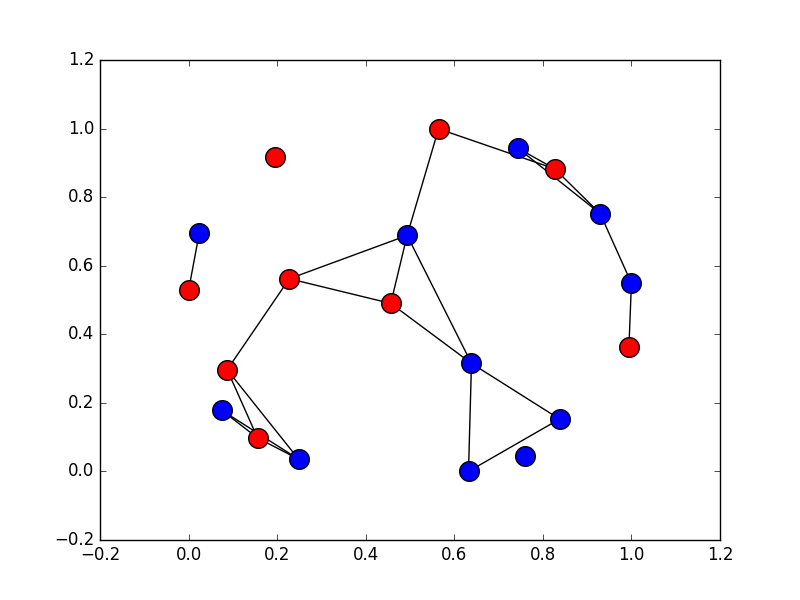
\includegraphics[scale=0.55]{anya.jpg}
  
  \caption{Reassignment of Centres}
\end{figure}
\end{flushleft}

We define ( the nodes labelled in Figure 4) as:
\begin{itemize}


\item Node type: $a$ : A centre in a partition which does not have edge to any boundary vertex.
\item Node type: $q$ : An interior non - centre, which is a client of $a$ and adjacent to a boundary vertex. We will call it the semi boundary vertex. 
\end{itemize} 
We observe that if we make as many semi-boundary centres as possible, such that they cover maximum number of boundary vertices, by shifting the centres located at $a$ to $q$ then we can come to a conclusion. 
If we make the semi-boundary vertex $q$ as a centre, then it will cover all the clients that have been covered by its respective centre $a$, but now the minimum maximum distance would be at most 4*OPT. Also, we would need to shift to such a set of semi-boundary vertices that maximises the number of distinct boundary vertices getting covered. So, we make a flow network for the same as shown in Figure 5.

\begin{flushleft}
\begin{figure}[H]
\includegraphics[scale=0.5]{diag3(2).jpg}
\caption{Flow to exchange Semi-boundary vertices with Existing Centres}
\end{figure}
\end{flushleft}
But we cannot make greedy moves and just move to the semi-boundary vertices with maximum boundary neighbours, as it is very necessary to make sure these boundary neighbours are distinct. To ensure this, we have Figure 6.
\begin{center}
\begin{figure}[H]
\includegraphics[scale=0.35]{diag4.jpg}
\caption{New Flow Method}
\end{figure}\end{center}
We keep the capacity of all edges in this flow network as 1 but modify the edge weights of edge weights between $B$, $Q$ and $A$ to keep a check. Between $A$ and $Q$, $e_1$ the remaining capacity of $q_i$ which is -- $L-$the number of non centres transferred to it through $a_i$ is taken as the edge weight between $q_i$ and $a_i$. While the edge weight between $B$ and $Q$, $e_2$ is equal to the inverse of the number of boundary vertices that the corresponding $q$ will cover if selected. 
\begin{center}
\begin{figure}[H]
\includegraphics[scale=0.3]{diag6.jpg}
\caption{Case of 2 Available Paths}
\end{figure}

\end{center}
\vspace{0.1cm}
In a case as shown above in Figure 7, if capacity permits, we will choose the path with $e_2 = 1/8$ as it the semi-boundary vertex involved is covering 7 other boundary vertices except the one in the selected augmented path. Also we will have to make changes to the edge weights like converting 1/4 to zero and the corresponding edges of the same semi boundary vertex involved to 1/3 and the semi-boundary to corresponding centre as 3. If later 1/8 weight wedge is not a part of the max flow then we simply revert back to the original weights.\\
But we realised that this problem of covering maximum number of boundary vertices is a problem reducible to the max-coverage problem, which is NP-hard. Hence the problem we are trying to solve is indeed NP-hard. The comparison is made by taking the nodes inside the partition as the subsets. (Figure 8)
\begin{center}
\begin{figure}[H]
\includegraphics[scale=0.55]{diag5.jpg}
\caption{Max-Coverage Problem}
\end{figure}
\end{center}
If there is a way where we can get minimum subsets to cover all of the universe then it is the same solution as we were trying to form which is not possible. However, we still feel that this idea of shifting centres to semi-boundary vertices could lead to some result. 
\end{itemize}
\subsection{Independent Trial}
In our attempt we start by applying the 2-approximation $K$-centre algorithm on the given graph. We then try to apply what we had learnt by reading the OPT + 1 local search algorithm of the min-degree spanning tree from section 2.6 of Williamson \& Shmoys. Effectively,if possible we transfer the load from the highest capacity nodes to lower ones through a contiguous sequence of edge assignment swaps until we reach a vertex with lower capacity as visible in the figure. \\
\begin{figure}[H]
\begin{center}
\includegraphics[scale=0.25]{d3.jpg}
  \caption{Reassignment Through Propagation}
  \label{Figure 13}
\end{center}
\end{figure}
\textbf{Algorithm:}
\begin{algorithmic}[1]
\STATE Start with $K'$ centres of $G^2$ with no regard to capacity $L$ using the 2-approximation algorithm for uncapacitated $K$-centre.
\STATE $C \leftarrow$ set of all $K$-centres
\STATE $C^l \leftarrow$ subset of $C$ such that$\forall C \in C^l$, $C$ covers exactly $l$ clients.
\STATE In each phase:\\
\STATE \hspace{1cm}$l \leftarrow$ the maximum degree of any centre\\
\STATE \hspace{1cm}$C_l \leftarrow$ set of all centres with degree $l$
\STATE Subphase
\WHILE {there are centre with degree $l$} 
\STATE Choose a client v assigned to some centre in $C_l$.
\STATE Choose any other centre $C_m$, preferably, of maximum residual capacity, and find a path as described in Figure 9 to $C_m$. Choose the path to $C_m$ having centre-client pairs such that we can do a series of edge swaps as described in Figure 9.
\ENDWHILE
\end{algorithmic}
This is done in order to reduce the maximum number of assignments to a particular centre so as to reach the capacity $L$. This propagation is possible only when a non centre is connected to two or more centres and hence reassignment can be done.\\
But we still might have too few centres in dense areas while just sufficient in other parts or maybe even having residual capacities in sparse areas. We also have a counterexample for the same as shown in Figure 10. The centres are represented by the rectangular marks on the vertices. The leftmost centre is covering many clients within a distance of $\leq 2$ whereas the situation is the other extreme i.e. too few clients for the other centres. Thus wasting their capacity.\\
\begin{figure}[H]
\begin{center}
\includegraphics[scale=0.25]{d1.jpg}
  \caption{Counterexample}
  \label{Figure 12}
\end{center}
\end{figure} Maybe moving to higher powers of $G$ may contribute to requiring less centres at regions where at present the centres are suffice.

Hence, from $G^2$ we move to $G^4$. Here, each centre with its clients forming a star graph will transform into a clique. The same is shown in Figure 11 below.\begin{figure}[H]
\begin{center}
\includegraphics[scale=0.45]{d2.jpg}
  \caption{Clique formation}
  \label{Figure 10}
\end{center}
\end{figure} With such a change we might be able to merge few cliques by placing a centre on a common node of two cliques(while removing their respective centres) such that both the cliques add up to give vertices less than L. 

Following this we have free centres available which we can place in dense cliques with high degree of vertices. Like in Figure 12, centres in $G^2$ are represented by square labels in the left figure and diamond label on the right while the one that replaces them in $G^4$ is represented by a square in the right figure.
\begin{figure}[H]
\begin{center}
\includegraphics[scale=0.3]{d4.jpg}
  \caption{Merging}
  \label{Figure 11}
\end{center}
\end{figure}
Why are we doing this? By doing the above $merging$ operation, we obtain an extra centre that can be placed at any location of our choice. The problem still remains on how to keep obtaining such centres other than by merging and then placing them at an appropriate position. We stop here.

Further, we tried to come up with some kind of data structure that might help us make some claims on the lower bound on K, when the edge reassignment operation stops at a local optima. \begin{figure}[H]
\includegraphics[scale=0.4]{diag8.jpg}
\caption{Level Structure}
\end{figure}
As shown above in Figure 13, we make a level structure with the set domains with centre $C_i$ by placing the domains of size $l$ at level $l$. This is the final structure after all reassignments which follows the upcoming theorems. Also edges $A,\: B \:, and \: C$ cannot be present.\\ We say it is the final structure because, after a reassignment operation, the set of neighbours of (more than or equal to 2) centres change, and also, their capacities change, thus moving them to different levels throughout the edge reassignment phase. \\\\\textbf{Theorem:}
When there can be no more edge reassignments, then no centre at level $l$ is within a distance $\leq 4$ to any node in level $l’ \geq l+2$ for all $l$. 
\\\\
\textbf{Proof:}This case is depicted in the level structure figure by edge $A$ in the level structure. After there can be no more reassignments, let there exists such a centre $C$ at a level $l$ which has an edge to some node P belonging to some level $l’ \geq l + 2$ i.e. let edge A exist. Let $C’$ be the centre covering the node $P$. Then we can do a reassignment step such that $P$ gets assigned to $C$ instead of $C`$ thereby moving $C`$ one level down and $C$ one level up. Thus the max degree can decrease this way removing one clique at a time. 

This contradicts our assumption that no more reassignment is possible.\\\\
\textbf{Theorem:} When there can be no more reassignments, if a centre $C_l$ at level $l$ is within distance $\leq$ 4 to a non-centre at level $l+1$, then any centre $C'< l$ at levels $< l$, will not be within a distance $\leq$4 from any node in the domain of $C_l$.\\\\
\textbf{Proof:}
This situation is represented by edge $B$ in the level structure. We will prove by contradiction. Let us say such a case exists, i.e., edge $B$ in the figure exists. Then, we can do a series of reassignments, to reduce the degree of a centre at $C_l$ at some level $\geq l + 1$. This is a contradiction, since we assumed in the beginning that we have reached at least a local optima and there can be no more reassignments.
\section{Bibliography}
\begin{enumerate}
\item Samir Khuller, and Yoram J. Sussmann, \textit{'The Capacitated K-Center Problem'}. 

\item Hyung-Chan An, Aditya Bhaskara, and Ola Svensson, \textit{'Centrality of Trees for Capacitated k-Center'}

\item David P. Williamson, and David B. Shmoys, 
\textit{The Design of Approximation Algorithms}
 
\item Vijay V. Vazirani, \textit{Approximation Algorithms}

\item Aounon Kumar, \textit{Network Location Problem Notes} (Work in Progress)
\end{enumerate}
\begin{appendices}
\section{The Integer Program}
\begin{center}

\begin{figure}[H]
 \includegraphics[scale=1.4]{1.png}
  
  \label{Figure 2}
\end{figure}

\begin{figure}[H]
 \includegraphics[scale=1.4]{2_1.png}
  
  \label{Figure 3}
\end{figure}

\end{center}
\section{Local Search Program}
\begin{flushleft}
\begin{figure}[H]
 \includegraphics[scale=1.4]{a.png}
  
  \label{Figure 4}
\end{figure}

\begin{figure}[H]
 \includegraphics[scale=1.4]{b.png}
  
  \label{Figure 5}
\end{figure}

\begin{figure}[H]
 \includegraphics[width=17cm,height=25cm]{c.png}
  
  \label{Figure 6}
\end{figure}
\begin{figure}[H]
 \includegraphics[width=17cm,height=25cm]{d.png}
  
\end{figure}
\begin{figure}[H]
 \includegraphics[width=10cm,height=5cm]{e.png}
  
\end{figure}
For the randomized local search we modify the getVmax function in the above code as:

\begin{figure}[H]
 \includegraphics[width=17cm,height=17cm]{f.png}
  
\end{figure}
\end{flushleft}
\section{Random Graph Generation}
This is the code snippet from the program it was used in:
\begin{figure}[H]
 \includegraphics[scale=1.2]{prajwal.png}
  
  \label{Figure 7}
\end{figure}
\section{Star Graph Generation}
\begin{figure}[H]
 \includegraphics[scale=1.3]{g1.png}
 
  \label{Figure 8}
\end{figure}

\begin{figure}[H]
\includegraphics[width=17cm,height=25cm]{g2.png}
  
  \label{Figure 9}
\end{figure}
\section{Unit Square Graph Generation}
\begin{figure}[H]
 \includegraphics[width=17cm,height=23cm]{us.png}
 
  \label{Figure 8}
\end{figure}

\end{appendices}

\end{document}
